\documentclass[border=4pt]{standalone}
\usepackage{amsmath,amssymb}
\usepackage{tikz}
\usetikzlibrary{arrows.meta,calc}
\newcommand{\bx}[6]{\draw[#5] (#1,#2) rectangle (#3,#4);
  \node[anchor=north west, text width=\dimexpr #3cm-#1cm-0.4cm\relax, align=left, font=\footnotesize, inner sep=0pt] at ({#1+0.2},{#4-0.18}) {#6};}
\tikzset{
 base/.style={rounded corners=3pt, line width=0.5pt},
 learn/.style={base, draw=red!60!black, fill=red!5},
 brain/.style={base, draw=violet!70!black, fill=violet!8},
 tank/.style={base, draw=teal!60!black, fill=teal!8},
 ledger/.style={base, draw=teal!60!black, dashed, fill=teal!3},
 hand/.style={base, draw=orange!70!black, dashed, fill=orange!3},
 handin/.style={base, draw=orange!70!black, fill=orange!12},
 cons/.style={base, draw=blue!60!black, fill=blue!7},
 grt/.style={base, draw=gray!70!black, fill=gray!8},
 plant/.style={base, draw=black!70, fill=gray!18},
 env/.style={base, draw=black!70, dashed, fill=gray!6},
 sig/.style={-{Latex[length=2.2mm]}, line width=0.6pt},
 nrg/.style={-{Latex[length=2.2mm]}, line width=0.9pt, teal!60!black},
 wup/.style={-{Latex[length=2.2mm]}, line width=0.7pt, dashed, red!60!black},
 lab/.style={font=\scriptsize, inner sep=1.5pt}
}
\begin{document}
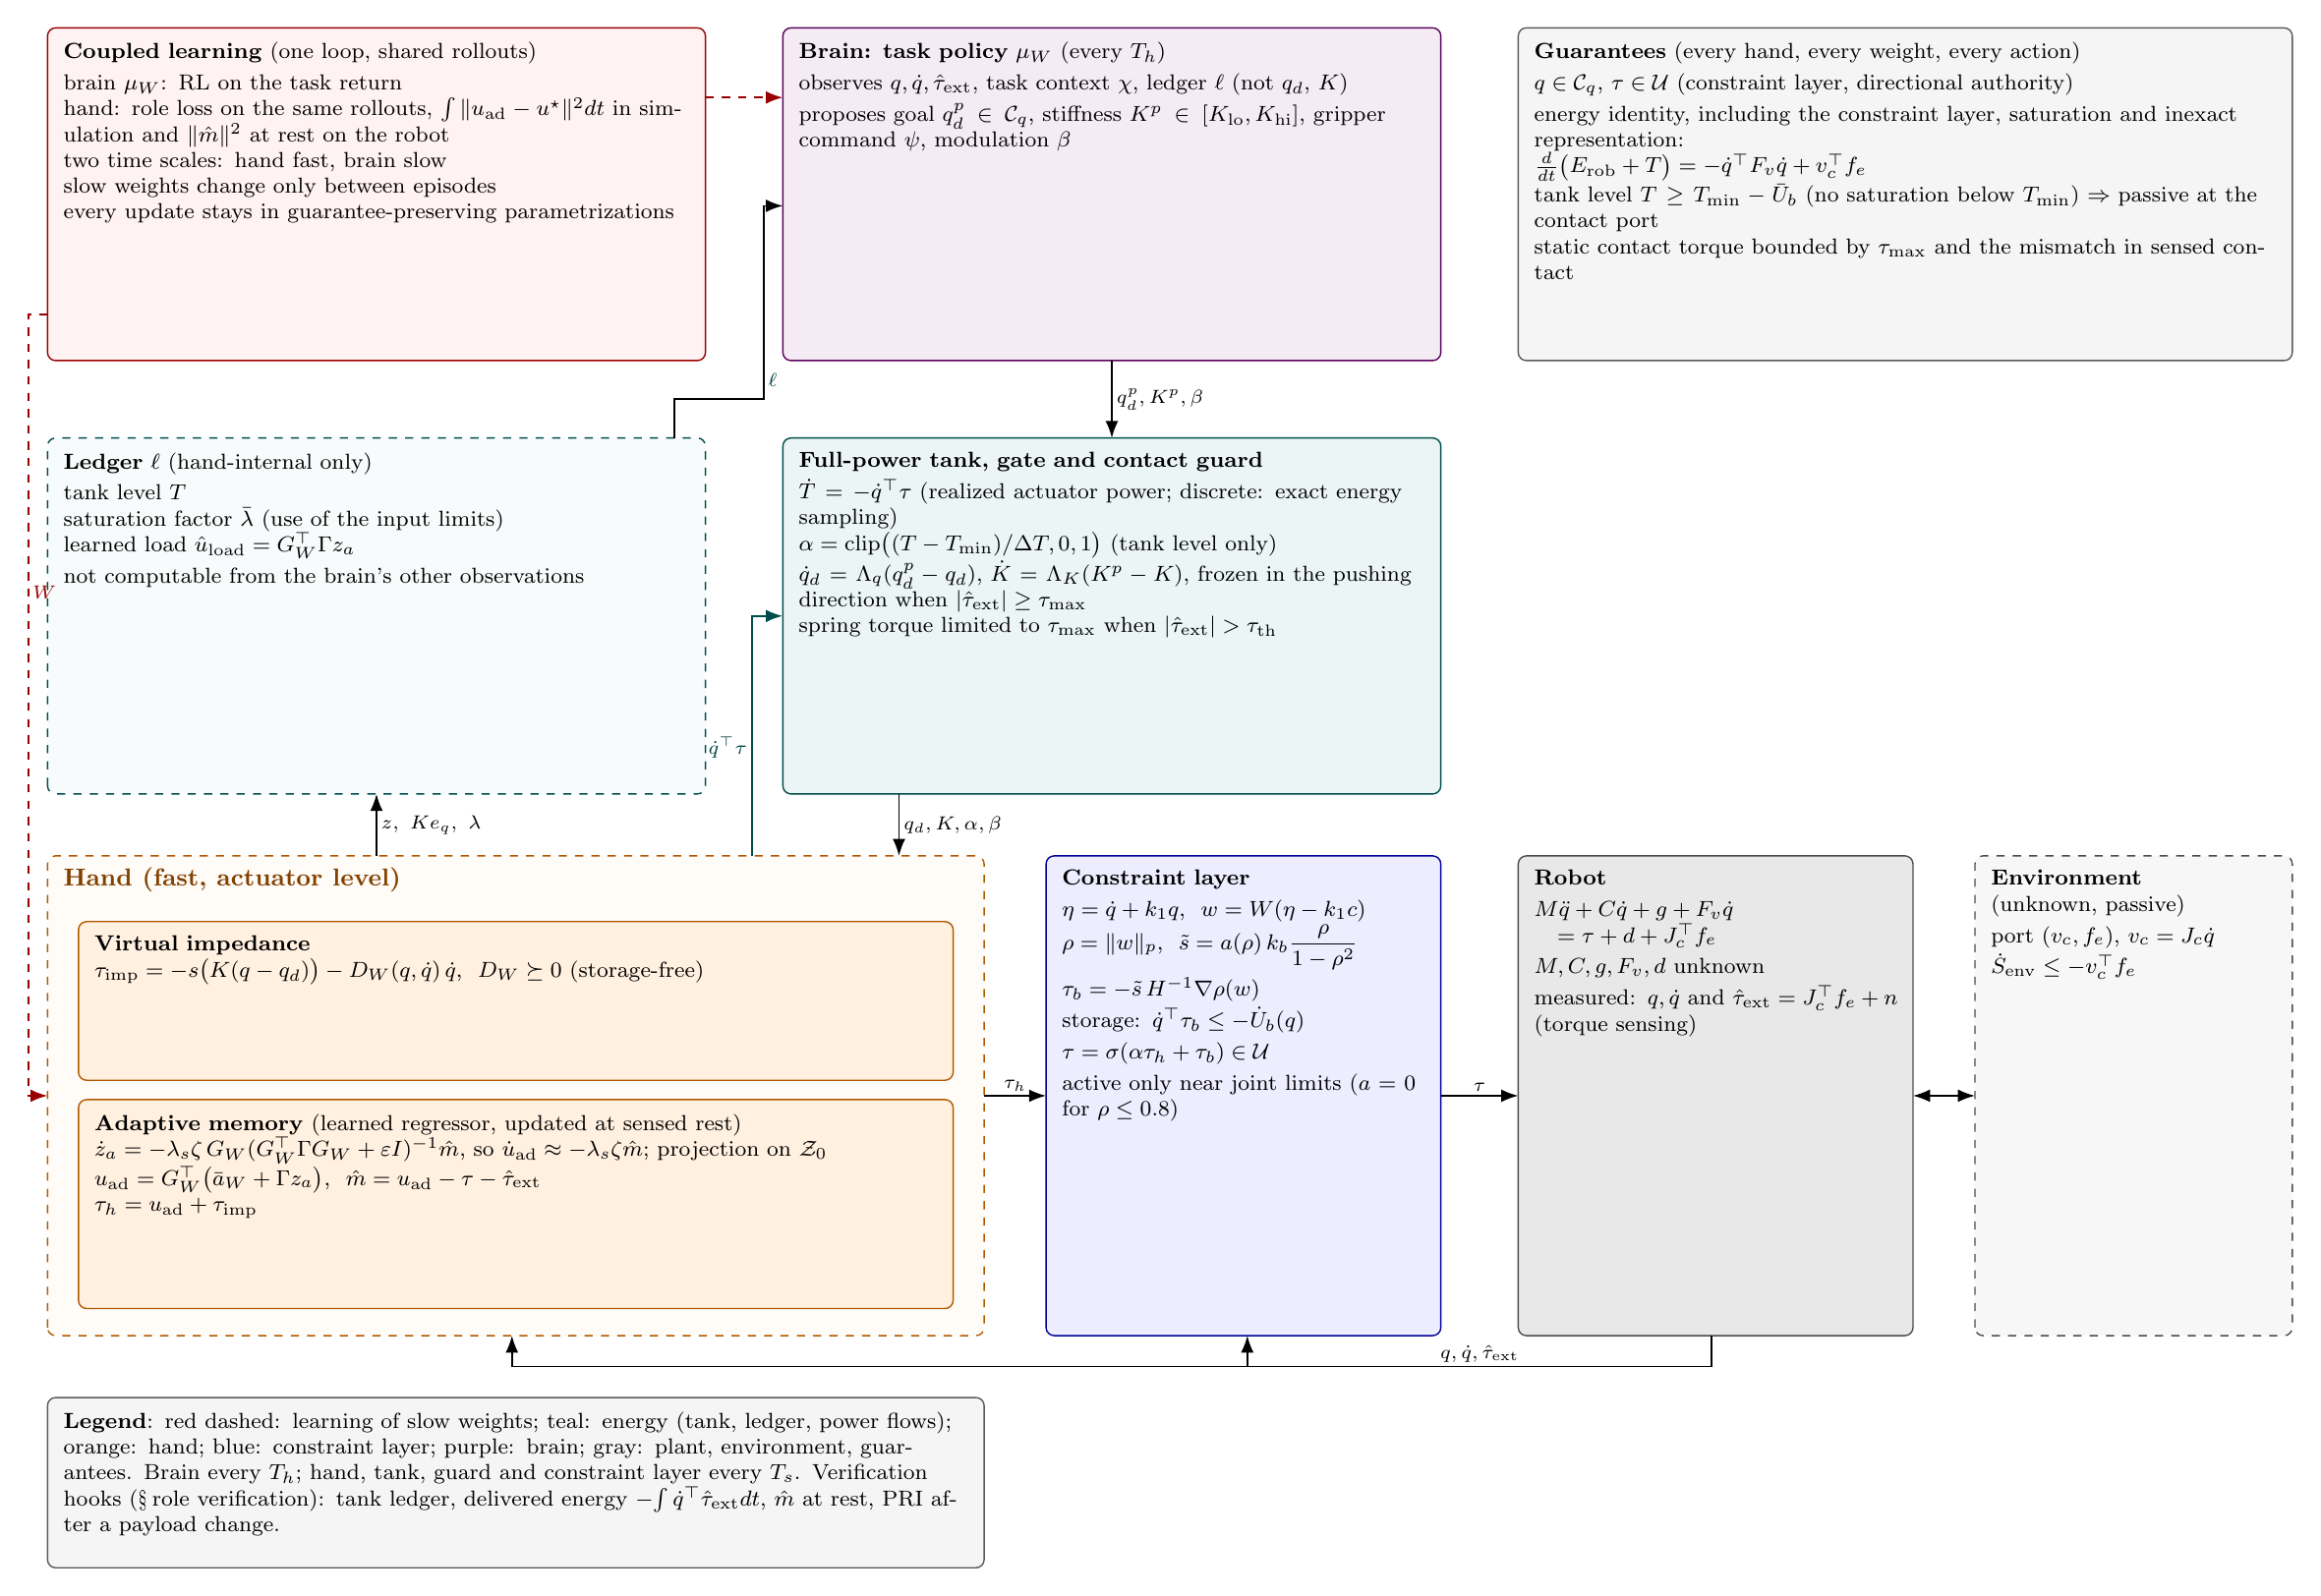
\begin{tikzpicture}[x=1cm,y=1cm]
\bx{0.5}{16.0}{9.0}{20.3}{learn}{\textbf{Coupled learning} (one loop, shared rollouts)\\[2pt]
brain $\mu_W$: RL on the task return\\
hand: role loss on the same rollouts, $\int\|u_{\mathrm{ad}}-u^\star\|^2dt$ in simulation and $\|\hat m\|^2$ at rest on the robot\\
two time scales: hand fast, brain slow\\
slow weights change only between episodes\\
every update stays in guarantee-preserving parametrizations}
\bx{10.0}{16.0}{18.5}{20.3}{brain}{\textbf{Brain: task policy $\mu_W$} (every $T_h$)\\[2pt]
observes $q,\dot q,\hat\tau_{\mathrm{ext}}$, task context $\chi$, ledger $\ell$ (not $q_d$, $K$)\\[2pt]
proposes goal $q_d^p\in\mathcal C_q$, stiffness $K^p\in[K_{\mathrm{lo}},K_{\mathrm{hi}}]$, gripper command $\psi$, modulation $\beta$}
\bx{19.5}{16.0}{29.5}{20.3}{grt}{\textbf{Guarantees} (every hand, every weight, every action)\\[2pt]
$q\in\mathcal C_q$, $\tau\in\mathcal U$ (constraint layer, directional authority)\\[2pt]
energy identity, including the constraint layer, saturation and inexact representation:\\
$\tfrac{d}{dt}\big(E_{\mathrm{rob}}+T\big)=-\dot q^\top F_v\dot q+v_c^\top f_e$\\
tank level $T\ge T_{\min}-\bar U_b$ (no saturation below $T_{\min}$) $\Rightarrow$ passive at the contact port\\
static contact torque bounded by $\tau_{\max}$ and the mismatch in sensed contact}
\bx{0.5}{10.4}{9.0}{15.0}{ledger}{\textbf{Ledger $\ell$} (hand-internal only)\\[2pt]
tank level $T$\\
saturation factor $\bar\lambda$ (use of the input limits)\\
learned load $\hat u_{\mathrm{load}}=G_W^\top\Gamma z_a$\\[2pt]
not computable from the brain's other observations}
\bx{10.0}{10.4}{18.5}{15.0}{tank}{\textbf{Full-power tank, gate and contact guard}\\[2pt]
$\dot T=-\dot q^\top\tau$ (realized actuator power; discrete: exact energy sampling)\\
$\alpha=\mathrm{clip}\big((T-T_{\min})/\Delta T,0,1\big)$ (tank level only)\\
$\dot q_d=\Lambda_q(q_d^p-q_d)$, $\dot K=\Lambda_K(K^p-K)$, frozen in the pushing direction when $|\hat\tau_{\mathrm{ext}}|\ge\tau_{\max}$\\
spring torque limited to $\tau_{\max}$ when $|\hat\tau_{\mathrm{ext}}|>\tau_{\mathrm{th}}$}
\bx{0.5}{3.4}{12.6}{9.6}{hand}{}
\node[anchor=north west, font=\small\bfseries, inner sep=0pt, orange!50!black] at (0.7,9.45) {Hand (fast, actuator level)};
\bx{0.9}{6.7}{12.2}{8.75}{handin}{\textbf{Virtual impedance}\\
$\tau_{\mathrm{imp}}=-s\big(K(q-q_d)\big)-D_W(q,\dot q)\,\dot q$, \ $D_W\succeq0$ (storage-free)}
\bx{0.9}{3.75}{12.2}{6.45}{handin}{\textbf{Adaptive memory} (learned regressor, updated at sensed rest)\\
$\dot z_a=-\lambda_s\zeta\,G_W(G_W^\top\Gamma G_W+\varepsilon I)^{-1}\hat m$, so $\dot u_{\mathrm{ad}}\approx-\lambda_s\zeta\hat m$; projection on $\mathcal Z_0$\\
$u_{\mathrm{ad}}=G_W^\top\big(\bar a_W+\Gamma z_a\big)$, \ $\hat m=u_{\mathrm{ad}}-\tau-\hat\tau_{\mathrm{ext}}$\\
$\tau_h=u_{\mathrm{ad}}+\tau_{\mathrm{imp}}$}
\bx{13.4}{3.4}{18.5}{9.6}{cons}{\textbf{Constraint layer}\\[2pt]
$\eta=\dot q+k_1q$, \ $w=W(\eta-k_1c)$\\
$\rho=\|w\|_p$, \ $\tilde s=a(\rho)\,k_b\dfrac{\rho}{1-\rho^2}$\\[2pt]
$\tau_b=-\tilde s\,H^{-1}\nabla\rho(w)$\\[2pt]
storage: $\dot q^\top\tau_b\le-\dot U_b(q)$\\[2pt]
$\tau=\sigma(\alpha\tau_h+\tau_b)\in\mathcal U$\\[2pt]
active only near joint limits ($a=0$ for $\rho\le0.8$)}
\bx{19.5}{3.4}{24.6}{9.6}{plant}{\textbf{Robot}\\[2pt]
$M\ddot q+C\dot q+g+F_v\dot q$\\ $\quad=\tau+d+J_c^\top f_e$\\[2pt]
$M,C,g,F_v,d$ unknown\\[2pt]
measured: $q,\dot q$ and $\hat\tau_{\mathrm{ext}}=J_c^\top f_e+n$ (torque sensing)}
\bx{25.4}{3.4}{29.5}{9.6}{env}{\textbf{Environment}\\(unknown, passive)\\[2pt]
port $(v_c,f_e)$, $v_c=J_c\dot q$\\[2pt]
$\dot S_{\mathrm{env}}\le-v_c^\top f_e$}
\bx{0.5}{0.4}{12.6}{2.6}{grt}{\textbf{Legend}: red dashed: learning of slow weights; teal: energy (tank, ledger, power flows); orange: hand; blue: constraint layer; purple: brain; gray: plant, environment, guarantees. Brain every $T_h$; hand, tank, guard and constraint layer every $T_s$. Verification hooks (\S\,role verification): tank ledger, delivered energy $-\!\int\dot q^\top\hat\tau_{\mathrm{ext}}dt$, $\hat m$ at rest, PRI after a payload change.}
\draw[sig] (14.25,16.0) -- (14.25,15.0) node[lab, midway, right] {$q_d^p,K^p,\beta$};
\draw[sig] (11.5,10.4) -- (11.5,9.6) node[lab, midway, right] {$q_d,K,\alpha,\beta$};
\draw[nrg] (9.6,9.6) -- (9.6,12.7) -- (10.0,12.7);
\node[lab, teal!50!black, left] at (9.6,11.0) {$\dot q^\top\tau$};
\draw[sig] (4.75,9.6) -- (4.75,10.4) node[lab, midway, right] {$z,\ K e_q,\ \lambda$};
\draw[sig] (8.6,15.0) -- (8.6,15.5) -- (9.75,15.5) -- (9.75,18.0) -- (10.0,18.0);
\node[lab, teal!50!black, right] at (9.75,15.75) {$\ell$};
\draw[sig] (12.6,6.5) -- (13.4,6.5) node[lab, midway, above] {$\tau_h$};
\draw[sig] (18.5,6.5) -- (19.5,6.5) node[lab, midway, above] {$\tau$};
\draw[{Latex[length=2.2mm]}-{Latex[length=2.2mm]}, line width=0.6pt] (24.6,6.5) -- (25.4,6.5);
\draw[sig] (22.0,3.4) -- (22.0,3.0) -- (6.5,3.0) -- (6.5,3.4);
\draw[sig] (16.0,3.0) -- (16.0,3.4);
\node[lab, above] at (19.0,3.0) {$q,\dot q,\hat\tau_{\mathrm{ext}}$};
\draw[wup] (9.0,19.4) -- (10.0,19.4);
\draw[wup] (0.5,16.6) -- (0.25,16.6) -- (0.25,6.5) -- (0.5,6.5);
\node[lab, red!60!black, right] at (0.25,13.0) {$W$};
\end{tikzpicture}
\end{document}
